%-*-coding: utf-8-*-

\chapter{Описание технических аспектов реализации}
В данной главе будут представлены технические аспекты реализации лямбд и анонимных функций.
Будет показана инженерная сложность и примененные подходы при решении поставленной задачи.

\section{Общий принцип работы}
Рассмотрим общий принцип работы KPHP и его архитектуру и попробуем решить как правильно подходить к решению данной задачи.
KPHP - состоит из двух основных частей:
\begin{enumerate}
\item компилятор - который занимается разбором написанного кода, построением абстрактного синтаксического дерева, анализом, трансляцией и выступает в качестве драйвера для компиляции оттранслированной программы;
\item рантайм - библиотека необходимая для запуска скомпилированных программ, содержащая скомпилированные встроенные функции языка.
\end{enumerate}

\subsection{Принцип работы компилятора}
Компилятор запускается с 24 рабочими потоками, для ускорения выполнения работ, большинство из этапов конвейера работают параллельно, что значительно уменьшает время выполнения.
На рисунке \ref{fig:compiler_arch} наглядно показана упрощенная схема основных этапов работы.
Если переход между этапами обозначен стрелочкой - это значит, что результат от предыдущего этапа сразу же передается на следующий.
Переходы же имеющие круглый конец означают, что мы должны дождаться выполнения всех предыдущих этапов во всех потоках выполнения перед тем как продолжить.

\begin{figure}[H]
    \caption{Общий принцип работы компилятора}
    \label{fig:compiler_arch}
    \centering
    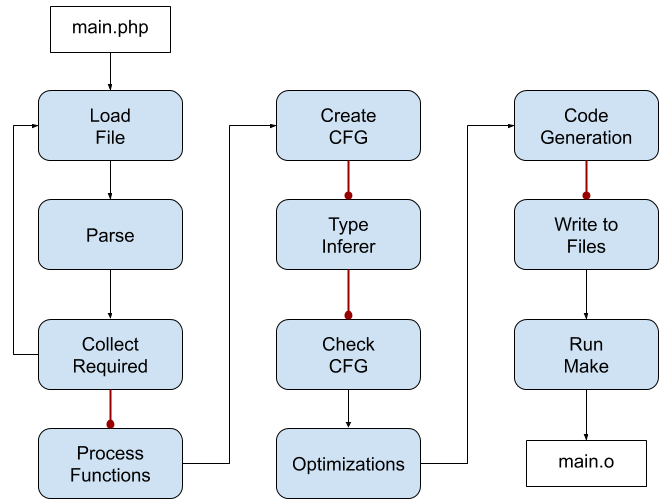
\includegraphics[width=\linewidth]{images/compiler_arch}
\end{figure}

Помимо множества аргументов, которые передаются на вход при запуске компилятора, нас будет интересовать только один - это путь к файлу, который является отправной точкой для компиляции.
Данный файл передается в начало конвейера, на рисунке \ref{fig:compiler_arch} - это файл с именем <<\verb|main.php|>>.
На этапе <<\verb|Load File|>> мы полностью загружаем переданный нам файл в память для дальнейшего разбора и анализа.
После чего у нас происходит разбиение его на токены и построение из них абстрактного синтаксического дерева для конкретного потока символов.
Имея построенное дерево разбора мы можем понимать какие вершины у нас встречаются и без труда выявляем все зависимости, которые нам будут необходимы для дальнейшей работы.
Каждый файл, который является зависимостью для предыдущего пришедшего файла отправляется снова на стадию <<\verb|Load File|>> и все этапы повторяются с самого начала.

На вход следующего шага нам уже передаются только разобранные функции.
При прохождении через <<\verb|Process Functions|>>  функций одна из основных задач расставить всем вершинам, соответствующим вызову другой функции, необходимые идентификаторы.
Это важный этап к которому уже должны быть разобраны все функции из других файлов, чтобы суметь проставить ссылки. Далее у нас происходит построение CFG \cite{CFG}, необходимого для дальнейшего анализа и оптимизаций.

Вывод типов для переменных, параметров функций, а также возвращаемых значений, происходит на шаге <<\verb|Type Inferer|>>.
В этот момент компилятор использует специальный файл - <<\verb|functions.txt|>>, содержащий аннотирование встроенных функции, которые необходимы программистам на языке KPHP.
Так как мы не имеем тела самих функций, мы вынуждены вводить свою аннотацию в этом случае.
Вывод типов в этом случае опирается на то, что написано в этом файле.
Дальше мы проверяем корректность и различные ограничения используя построенный CFG и выведенные типы у вершин и пытаемся оптимизировать на уровне AST наши функции.

После основных этапов мы получаем готовые деревья AST для всех функций.
Необходимо сгенерировать их в текстовое представление для последующей записи в файлы.
Учитывая выведенные типы мы должны там где необходимо печатать соответствующие типы выражений, а также в зависимости от вида вершины преобразовать в соответствующий код на языке C++.
Далее уже готовое текстовое представление распределенное по файлам необходимо записать на диск с нужным распределением по директориям для ускорения дальнейшей сборки.

Последний из основных этапов, который мы рассмотрим - это <<\verb|Run Make|>>.
На данном этапе мы смотрим на времена изменений файлов и понимаем какие зависимости нужно пере собрать.
Сборка происходит в несколько этапов:
\begin{enumerate}
  \item компиляция одной единицы трансляции;
  \item многопоточная линковка независимых групп бинарных файлов;
  \item линковка всех промежуточно слинкованных файлов в один исполняемый файл.
\end{enumerate}

На текущий момент мы должны уже получить исполняемый файл, который нуждается только в библиотеке с реализациями всех встроенных методов и содержащей всю необходимую функциональность для работы программы.

\subsection{Устройство рантайма}
\label{sec2:runtime_principle}
У созданного кода компилятором, есть несколько шагов которые необходимо выполнить в рантайме для запуска.
Среда выполнения содержит в себе функцию \verb|main| с которой начинается выполнение скрипта.
Там происходит инициализация необходимых глобальных констант, которые сгенерировал компилятор.
Проставляют необходимые функции для запуска и чистки памяти, по завершении.

Также библиотека рантайма содержит все нехватающие символы для резолвинга в собранном исполняемом файле.
Они все пишутся на C++ с нужными типами указанными в файле, который мы уже встречали - <<\verb|functions.txt|>>.
Все функции начинаются с префикса \verb|f$| и имеют типы такие, какие указаны в аннотации к функции.
Если например функция принимает параметр, имеющий тип \verb|Any| - то такая функция должна иметь шаблонную сигнатуру \cite[с.~665]{Stroustrup}.

Для большинства примитивных типов участвующих в работе программы написаны соответствующие обертки.
Так например есть реализация строк, которая поддерживает необходимую COW \cite{COW} семантику и весь набор используемой функциональности, такой как: конкатенация строк, удаление подстроки, взятие конкретного символа и так далее.
Также имеется реализация PHP массивов, которые по совместительству являются словарями.

Так как мы имеем дело с динамически типизированным языком, то у нас есть желание и право сохранять значения разных типов в одну и туже переменную.
Для этого был написан класс \verb|var|, который является типом-суммой и может содержать в себе любой из приметивных типов.
Также есть возможность превращать его обратно в строку, число, массив.
Такой класс имеет несколько проблем, связанных с производительностью, так как нам каждый раз нужно приводить его к специальному типу и проверять был ли он таковым.
Данный тип не может содержать пользовательские структуры по очень простой причине - их очень много для того, чтобы поддерживать такой тип, который мог бы хранить любой из экземпляров классов.
А создавать общий тип от которого наследовались бы все остальные классы - накладно с точки зрения производительности и потребления памяти.
Как минимум мы начнем потреблять на 8 байт больше при создании любого класса и при обращении мы будем вынуждены приводить его обратно.
Такое стало возможно при появлении интерфейсов созданных в ходе написания данной работы, но там программист явно понимает возможные недостатки при их использовании.

Все пользовательские структуры у нас хранятся отдельно в файле и представляют собой обычные C++ классы.
Методы имеющиеся в классе выносятся как глобальные функции, принимающие \verb|$this| первым параметром.
У данного подхода есть свои преимущества и недостатки.
С одной стороны это вносит небольшую неясность с первого взгляда и непонимания какие методы связаны с каким классом - в сгенерированном коде.
С другой стороны данный подход хорош тем, что все методы класса независимы и лежат в отдельных единицах трансляции, а при изменении сигнатуры одного из методов мы не будем вынуждены компилировать снова весь класс и все его методы.
Таким образом мы заключаем, что данный подход является оправданным решением в текущей архитектуре реализации пользовательских классов.

\section{Анонимные функции}
В данной главе посмотрим на анонимные функции и получившееся решение.
Полноценная реализация лямбд будет состоять из нескольких этапов:
\begin{enumerate}
  \item сначала нам нужно разобрать синтаксис и построить из этого AST;
  \item после необходимо расставить нужные ссылки на вызовы лямбды с соответствующими типами;
  \item понять как правильно вывести типы, учитывая разработанную аннотацию;
  \item сгенерировать необходимый класс и метод на этапе трансляции.
\end{enumerate}

\subsection{Разбор синтаксиса}
Сначала нам нужно превратить набор символов в более удобный формат для построения AST - набор токенов.
Этой задачей занимается лексер при помощи утилиты \verb|gperf| \cite[с.~461]{cpp_gems_gperf}, не будем вдаваться подробности его работы, а лучше рассмотрим на примере, что у нас получится после прохождения небольшого кода через лексер.
В листинге \ref{lst:pass_to_lexer} приведен пример и в комментариях указаны какие токены получаются на выходе лексера.
Осталось только разобраться, как из этого набора токенов построить абстрактное синтаксическое дерево.

\begin{lstlisting}[caption={Результат работы лексера},label={lst:pass_to_lexer}]
function ($x)     # tok_function tok_oppar tok_var  tok_clpar
  use ($y)        # tok_use      tok_oppar tok_var  tok_clpar
{                 # tok_opbrc
  return $x + $y  # tok_return   tok_var   tok_plus tok_var
  ;               # tok_semicolon
};                # tok_clbrc    tok_semicolon
\end{lstlisting}

Разбор данного набора будет происходить методом рекурсивного спуска \cite{recursive_descent_parser}.
При построении дерева, надо не забыть о всех проверках и выдать их в форме понятной для пользователя.
На выходе у нас получится абстрактное синтаксическое дерево, приведенное на рисунке \ref{fig:AST_for_id}.

\begin{figure}[H]
    \caption{AST для функции из листинга \ref{lst:pass_to_lexer}}
    \label{fig:AST_for_sum}
    \centering
    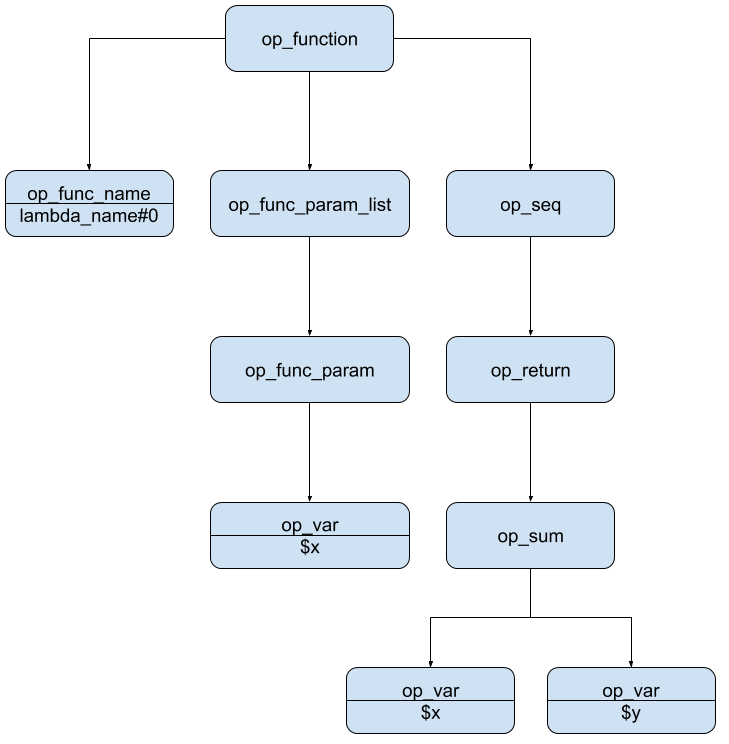
\includegraphics[width=\linewidth]{images/ast_for_id}
\end{figure}

Так как каждая анонимная функция должна иметь уникальное имя, будем его генерировать по такому алгоритму:
\begin{itemize}
  \item возьмем имя текущей функции, которую мы обрабатываем;
  \item посчитаем от нее хеш-функцию;
  \item заведем для каждой функции индивидуальный счетчик, возьмем следующее число;
  \item наше имя будет конкатенацией результата хеш-функции и нового числа из счетчика.
\end{itemize}

Такой подход нам позволяет без блокировок в других потоках, создавать уникальные для всей программы имена анонимных функций.
Когда мы получили AST для нашей анонимной функции, теперь надо придумать, куда и как его преобразовывать для дальнейшей работы.

\subsection{Шаблонные функции}
Так как язык KPHP транслируется в строго типизированный язык, нам нужно придумать механизм для реализации функций высших порядков.
В текущий момент, как было показано в \ref{sec2:runtime_principle}, мы не можем сохранять в одну переменную экземпляры разных классов, то нам нужно придумать механизм благодаря которому мы могли бы передавать экземпляры разных классов в одну переменную.


\subsection{Вывод типов}
Рассмотрим как у нас должен происходить вывод типов.
Все параметры лямбда-функции имеют шаблонный тип - об этом будет рассказано дальше.
Добавим в язык KPHP подсказку для параметров функции - \verb|callable|.
Она будет означать, что мы можем принять любую лямбда-функцию, либо класс у которого есть метод \verb|__invoke|.
Но по факту анонимная функция представляет из себя класс у которого есть метод \verb|__invoke| у которого все аргументы шаблонные.

Так как шаблонные функции будут рассмотрены дальше, нас будет интересовать как выводятся типы результата вызова лямбда-функции и типы во встроенных функциях.
Так как все вызовы лямбда функции транслируются просто в вызов соответствующего метода, то тут все заработает из коробки.
KPHP умел до этого сам выводить типы для вызова методов конкретного класса.
Но нужно добавить поддержку для встроенных методов.

Теперь разработаем аннотацию для встроенных функций.
Рассмотрим например функцию \verb|array_reduce($array, $callback, [$initial])| - такая функция, которая принимает массив, функцию с помощью которой она будет выполнять левоассоциативную свертку \cite{foldl} и начальное значение.
Например \verb|array_reduce([1, 2], sum, 10);| - возьмет начальное значение 10 и добавит к нему по очереди элементы массива один и два, в результате получим число 13.

Данная функция принимает первым аргументов массив каких-либо значений, запишем это в следующем виде: \verb|array<Any>|.
Следующий аргумент это другая функция, попробуй подумать какой у нее может быть тип:
\begin{enumerate}
  \item первый аргумент ее может принимать начальное значение, передаваемое третьим аргументом;
  \item первый аргумент может принимать значения, которая вернула сама функция свертки;
  \item вторым аргументом она всегда принимает значения из переданного массива;
  \item возвращает любое значение.
\end{enumerate}

Формализуем описанные выше требования.
Введем по аналогии с PHP ключевое слово для типа принимаемой функции - \verb|callback|.
Функция которую мы принимаем для свертки будет выглядеть следующим образом: \verb|callback($carry, $item) ::: Any|.
Синтаксис \verb|:::| - ограничивает выражение стоящее слева от него соответствующим типом, то есть наша функция может вернуть все что угодно.
Параметр \verb|$carry| будет иметь тип \verb|lca<^3, ^2()>|.
Слово \verb|lca| в данном контексте означает такой тип, который может содержать любые значения, из типа \verb|^3| и типа \verb|^2()|.
\verb|^3| - это ссылка на 3 аргумент функции, формально она говорит возьми тот тип который имеет третий аргумент функции \verb|array_reduce| в данном случае это будет тип переменной \verb|$initial|.
Тип результата вызовы функции обозначим как \verb|^2()| - это результат вызова функции передаваемой вторым аргументом, то есть функции для свертки.
Также наша функция принимает аргумент \verb|$item|, который будет иметь тип такой же как и элемент массива, то есть \verb|^1[]|.

Нам осталось только добавить тип для переменной задающей начальное значение - \verb|$initial|, так как она может быть какой угодно то ей зададим тип \verb|Any|.
А возвращаемый тип всей функции будет такой же, какой имеет параметр \verb|$carry| нашей функции, то есть \verb|lca<^3, ^2()>|.
Полный пример для указания типа функции \verb|array_reduce| представлен в листинге \ref{lst:typed_array_reduce}.

\begin{lstlisting}[caption={Пример типизации функции array\_reduce},label={lst:typed_array_reduce}]
function array_reduce(
  $a ::: array,
  callback($carry ::: lca<^3, ^2()>, $item ::: ^1[]) ::: Any,
  $initial ::: Any) ::: lca<^3, ^2()>;
\end{lstlisting}

Далее в качестве примера приведем типизации для нескольких встроенных функций \verb|array_filter| - листинг \ref{lst:typed_array_filter}, \verb|array_map| - листинг \ref{lst:typed_array_map} и \verb|usort| представлен в листинге \ref{lst:typed_usort}.

\begin{lstlisting}[caption={Пример типизации функции array\_filter},label={lst:typed_array_filter}]
function array_filter(
  $a ::: array,
  callback ($x ::: ^1[]) ::: bool = TODO) ::: ^1;
\end{lstlisting}

\begin{lstlisting}[caption={Пример типизации функции array\_map},label={lst:typed_array_map}]
function array_map(
  callback ($x ::: ^2[]) ::: Any,
  $a ::: array) ::: array <^1()>;
\end{lstlisting}

\begin{lstlisting}[caption={Пример типизации функции usort},label={lst:typed_usort}]
function usort(
  &$a ::: array,
  callback($x ::: ^1[], $y ::: ^1[]) ::: int) ::: void;

\end{lstlisting}

Для вывода типов, для начала нам нужно разобрать придуманный нами синтаксис и представить его в удобной форме.
Будем использовать \verb|enum-тип|, каждое значение которого обозначает какой-либо примитивный тип:
\begin{lstlisting}
enum PrimitiveType {
  tp_Unknown,
  tp_False,
  tp_bool,
  tp_int,
  tp_float,
  tp_array,
  tp_string,
  tp_void,
  tp_var,
  tp_Class,
  tp_Error,
  tp_Any,
};
\end{lstlisting}

Построим дерево обозначающее данный тип, например для функции \verb|array_map|, в которую передают только анонимную функцию:
\begin{lstlisting}[label={lst:array_map_typed_ast}]
function array_map(
  callback($x ::: ^2[]) ::: Any
) ::: array<^1()>;
\end{lstlisting}
Мы получим дерево, изображенное на рисунке \ref{fig:ast_for_callback}.
Строим обычное дерево для функции, оно представлено слева, для упрощения убраны лишние вершины.
В каждой вершине есть поле \verb|type_rule| которое заполняется по мере необходимости.
Так например мы видим, что возвращаемое значение функции \verb|array_map|, содержащиеся в поле \verb|type_rule| вершины \verb|op_function|, представляет из себя массив элементов, которые имеют тип такой же как и результат вызова первого параметра.

\begin{figure}[H]
    \caption{Дерево разбора для типизации функции из листинга \ref{lst:array_map_typed_ast}}
    \label{fig:ast_for_callback}
    \centering
    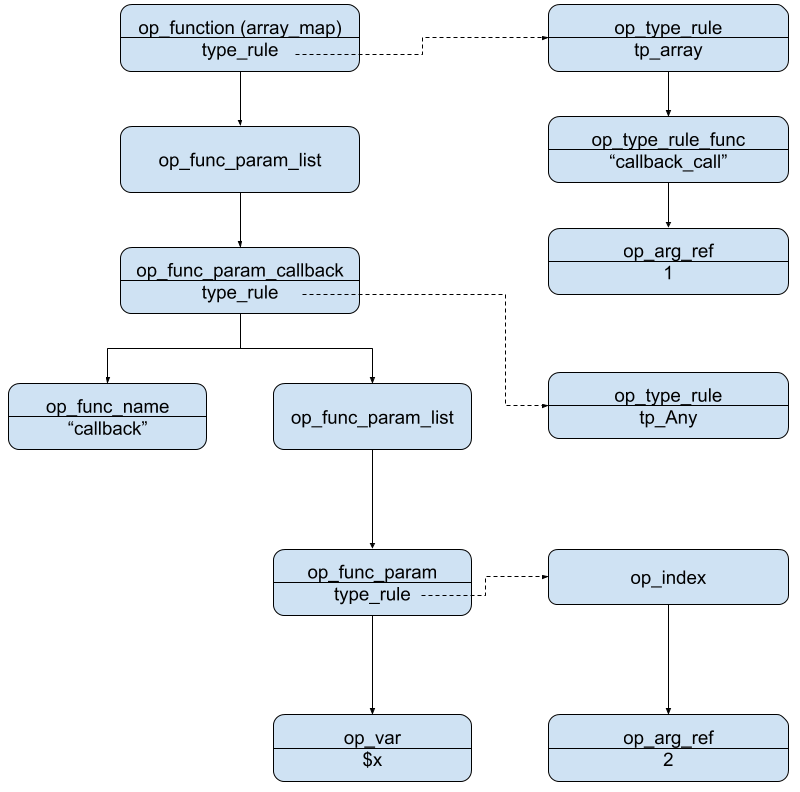
\includegraphics[width=\linewidth]{images/ast_for_callback}
\end{figure}

Осталось лишь встроить нужную логику в \verb|Type Inferer| (см. рисунок \ref{fig:compiler_arch}).
Во время вывода типов, для каждого выражения устанавливаются ограничения, что тип одного выражения должен иметь как минимум тип другого.
Например в выражении \verb|$x = foo();| мы ставим ограничение, что переменная должна иметь тип содержащий в себе множество значений не меньшее, чем множество содержащиеся в типе возвращаемого значения функции.
Таким образом, если в поле \verb|type_rule| мы видим, что это ``callback\_call'', содержащийся в вершине \verb|op_type_rule_func| - то мы должны достать нужный функциональный тип по порядковому номеру.
В текущее выражение мы будем накладывать ограничение, что оно должно иметь тип как минимум такой, какой имеет возвращаемое значение данной функции.

Также при задании типов аргументов \verb|callback|, надо наложить соответствующие ограничения.
То есть мы берем переданную нам функцию, достаем типы указанные в аннотации к функции и говорим, что данный параметр, переданной функции имеет как минимум такой тип.
Так же поступаем и с возвращаемым аргументом лямбда-функции.

\subsection{Кодогенерация}
В PHP один из магических методов в классе является \verb|__invoke|, если класс имеет этот метод, то PHP гарантирует, что при попытке вызвать экземпляр данного класса, передав ему аргументы он вызовет данный метод.
Лямбда-функции преобразовываются в соответствующей класс и глобальный метод \verb|__invoke|, который принимает в качестве первого аргумента экземпляр самой лямбда-функции.
Все захваченные переменные становятся полями данного класса.

Рассмотрим пример генерации функции, которая складывает передаваемое ей число и захваченную глобальную переменную:
\begin{lstlisting}[label={lst:sum_x_captured},caption={Пример функции добавляющей к аргументу захваченное значение}]
$y = 8;

$add_y = function ($x) use ($y) {
  return $x + $y;
};

$add_y(228);
\end{lstlisting}

Для лямбда-функции, приведенной в листинге \ref{lst:sum_x_captured} будет сгенерирован следующий класс:
\begin{lstlisting}
struct lambda1 final : refcountable_php_classes<lambda1> {
  int y;
};
\end{lstlisting}

Также будут сгенерированы глобальные методы для конструирования данной лямбда-функции и вызова соответствующего \verb|__invoke| метода:
\begin{lstlisting}
class_instance<lambda1> lambda1_construct(int y) {
  class_instance<lambda1> lambda1_this;
  lambda1_this.alloc();

  lambda1_this->y = y;
  return lambda1_this;
}

int lambda1_invoke_not_instance(class_instance<lambda1> const &lambda1_this, int x) {
  return x + lambda1_this->$y;
}
\end{lstlisting}

Код из листинга \ref{lst:sum_x_captured} будет преобразован, с использованием полученных классов и функций, в следующий:
\begin{lstlisting}
int y = 8;
class_instance<lambda1> id = lambda1_construct(y);
lambda1_invoke_not_instance(id, 228);
\end{lstlisting}

Данный подход генерации лямбда-функций удобен тем, что удачно вписывается в текущую архитектуру кодогенерации KPHP.

\section{Поддержка интерфейсов}
\subsection{Разбор синтаксиса}
\subsection{Генерация методов}
\subsection{Лямбды как члены классов}

\chapterconclusion
